% Szglab4
% ===========================================================================
%
\chapter{Grafikus felület specifikációja}

\thispagestyle{fancy}

\section{A grafikus interfész}

\Aref{fig:main}. ábra mutatja a főablakot, a benne lévő áramkör csak illusztráció. A két menü almenüi \aref{fig:menus}. ábrán látszódnak. A Fájl menü almenüi beszédesek, a felső három menüpontra megnyílik egy fájlválasztó ablak, ahol megadható egy fájl, majd az adott akció lefut. A Kilépés menüpont segítségével kiléphetünk az alkalmazásból. Az Egyéb menü Néjegy menüpontjára kapcsolva pedig megnyílik \aref{fig:about}. ábrán látható ablak.

\begin{figure}[h]
\begin{center}
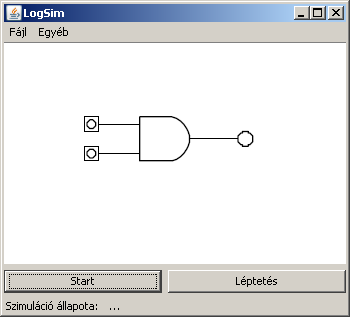
\includegraphics[width=4.25in]{chapters/chapter11/screenshots/felulet.png}
\caption{Főablak}
\label{fig:main}
\end{center}
\end{figure}

\begin{figure}[h]
\begin{center}
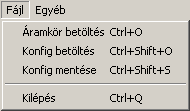
\includegraphics[width=1.98in]{chapters/chapter11/screenshots/menus1.png}
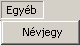
\includegraphics[width=0.83in]{chapters/chapter11/screenshots/menus2.png}
\caption{Fájl és az Egyéb menü almenüi}
\label{fig:menus}
\end{center}
\end{figure}

\begin{figure}[h]
\begin{center}
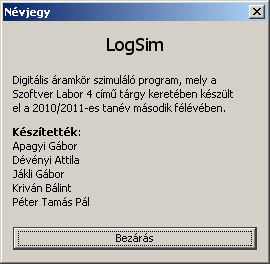
\includegraphics[width=2.8125in]{chapters/chapter11/screenshots/about.png}
\caption{Névjegy}
\label{fig:about}
\end{center}
\end{figure}

\section{A grafikus rendszer architektúrája}
\comment{A felület működésének elve, a grafikus rendszer architektúrája (struktúra diagramok). A struktúra diagramokon a prototípus azon és csak azon osztályainak is szerepelnie kell, amelyekhez a grafikus felületet létrehozó osztályok kapcsolódnak.}

\subsection{A felület működési elve}
\comment{Le kell írni, hogy a grafikai megjelenésért felelős osztályok, objektumok hogyan kapcsolódnak a meglevő rendszerhez, a megjelenítés során mi volt az alapelv. Törekedni kell az MVC megvalósításra. Alapelvek lehetnek: \textbf{push} alapú: a modell értesíti a felületet, hogy változott; \textbf{pull} alapú: a felület kérdezi le a modellt, hogy változott-e; \textbf{kevert}: a kettő kombinációja.}

\subsection{A felület osztály-struktúrája}
\comment{Osztálydiagram. Minden új osztály, és azon régiek, akik az újakhoz közvetlenül kapcsolódnak.}

\section{A grafikus objektumok felsorolása}
\comment{Az új osztályok felsorolása. Az régi osztályok közül azoknak a felsorolása, ahol változás volt. Ezek esetén csak a változásokat kell leírni.}

\subsection{Osztály1}
\begin{itemize}
\item Felelősség\newline
\comment{Mi az osztály felelőssége. Kb 1 bekezdés. Ha szükséges, akkor state-chart is.}
\item Ősosztályok\newline
\comment{Mely osztályokból származik (öröklési hierarchia)\newline
Legősebb osztály $\rightarrow$ Ősosztály2 $\rightarrow$ Ősosztály3...}
\item Interfészek\newline
\comment{Mely interfészeket valósítja meg.}
\item Attribútumok\newline
\comment{Milyen attribútumai vannak}
	\begin{itemize}
		\item attribútum1: attribútum jellemzése: mire való, láthatósága (UML jelöléssel), típusa
		\item attribútum2: attribútum jellemzése: mire való, láthatósága (UML jelöléssel), típusa
	\end{itemize}
\item Metódusok\newline
\comment{Milyen publikus, protected és privát  metódusokkal rendelkezik. Metódusonként precíz leírás, ha szükséges, activity diagram is  a metódusban megvalósítandó algoritmusról.}
	\begin{itemize}
		\item int foo(Osztály3 o1, Osztály4 o2): metódus leírása, láthatósága (UML jelöléssel)
		\item int bar(Osztály5 o1): metódus leírása, láthatósága (UML jelöléssel)
	\end{itemize}
\end{itemize}

\subsection{Osztály2}
\begin{itemize}
\item Felelősség\newline
\comment{Mi az osztály felelőssége. Kb 1 bekezdés. Ha szükséges, akkor state-chart is.}
\item Ősosztályok\newline
\comment{Mely osztályokból származik (öröklési hierarchia)\newline
Legősebb osztály $\rightarrow$ Ősosztály2 $\rightarrow$ Ősosztály3...}
\item Interfészek\newline
\comment{Mely interfészeket valósítja meg.}
\item Attribútumok\newline
\comment{Milyen attribútumai vannak}
	\begin{itemize}
		\item attribútum1: attribútum jellemzése: mire való, láthatósága (UML jelöléssel), típusa
		\item attribútum2: attribútum jellemzése: mire való, láthatósága (UML jelöléssel), típusa
	\end{itemize}
\item Metódusok\newline
\comment{Milyen publikus, protected és privát  metódusokkal rendelkezik. Metódusonként precíz leírás, ha szükséges, activity diagram is  a metódusban megvalósítandó algoritmusról.}
	\begin{itemize}
		\item int foo(Osztály3 o1, Osztály4 o2): metódus leírása, láthatósága (UML jelöléssel)
		\item int bar(Osztály5 o1): metódus leírása, láthatósága (UML jelöléssel)
	\end{itemize}
\end{itemize}

\section{Kapcsolat az alkalmazói rendszerrel}
\comment{Szekvencia-diagramokon ábrázolni kell a grafikus rendszer működését. Konzisztens kell legyen az előző alfejezetekkel. Minden metódus, ami ott szerepel, fel kell tűnjön valamelyik szekvenciában. Minden metódusnak, ami szekvenciában szerepel, szereplnie kell a valamelyik osztálydiagramon.}

\begin{figure}[h]
\begin{center}
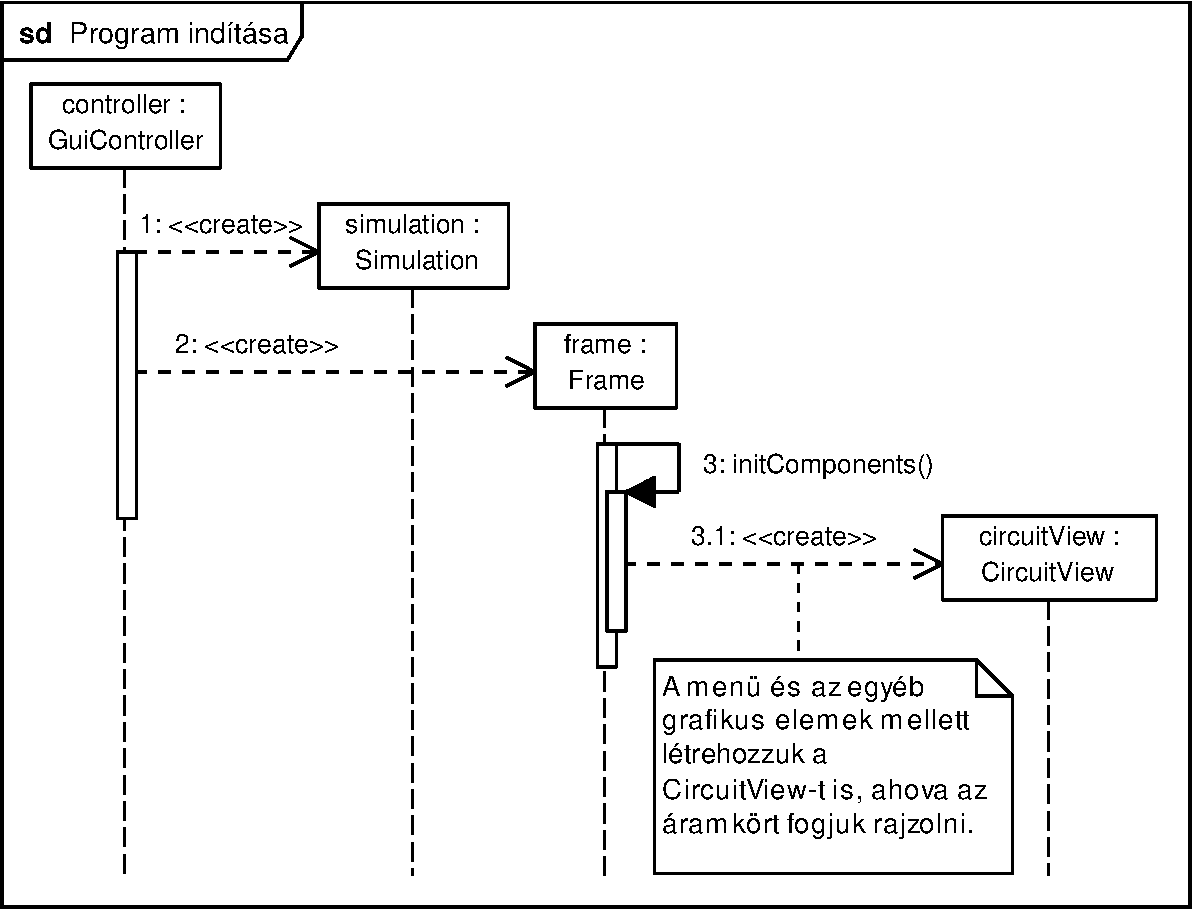
\includegraphics[width=17cm]{chapters/chapter11/pdfs/1_program_start.pdf}
\caption{Program indítása}
\label{fig:program_start}
\end{center}
\end{figure}

\begin{figure}[h]
\begin{center}
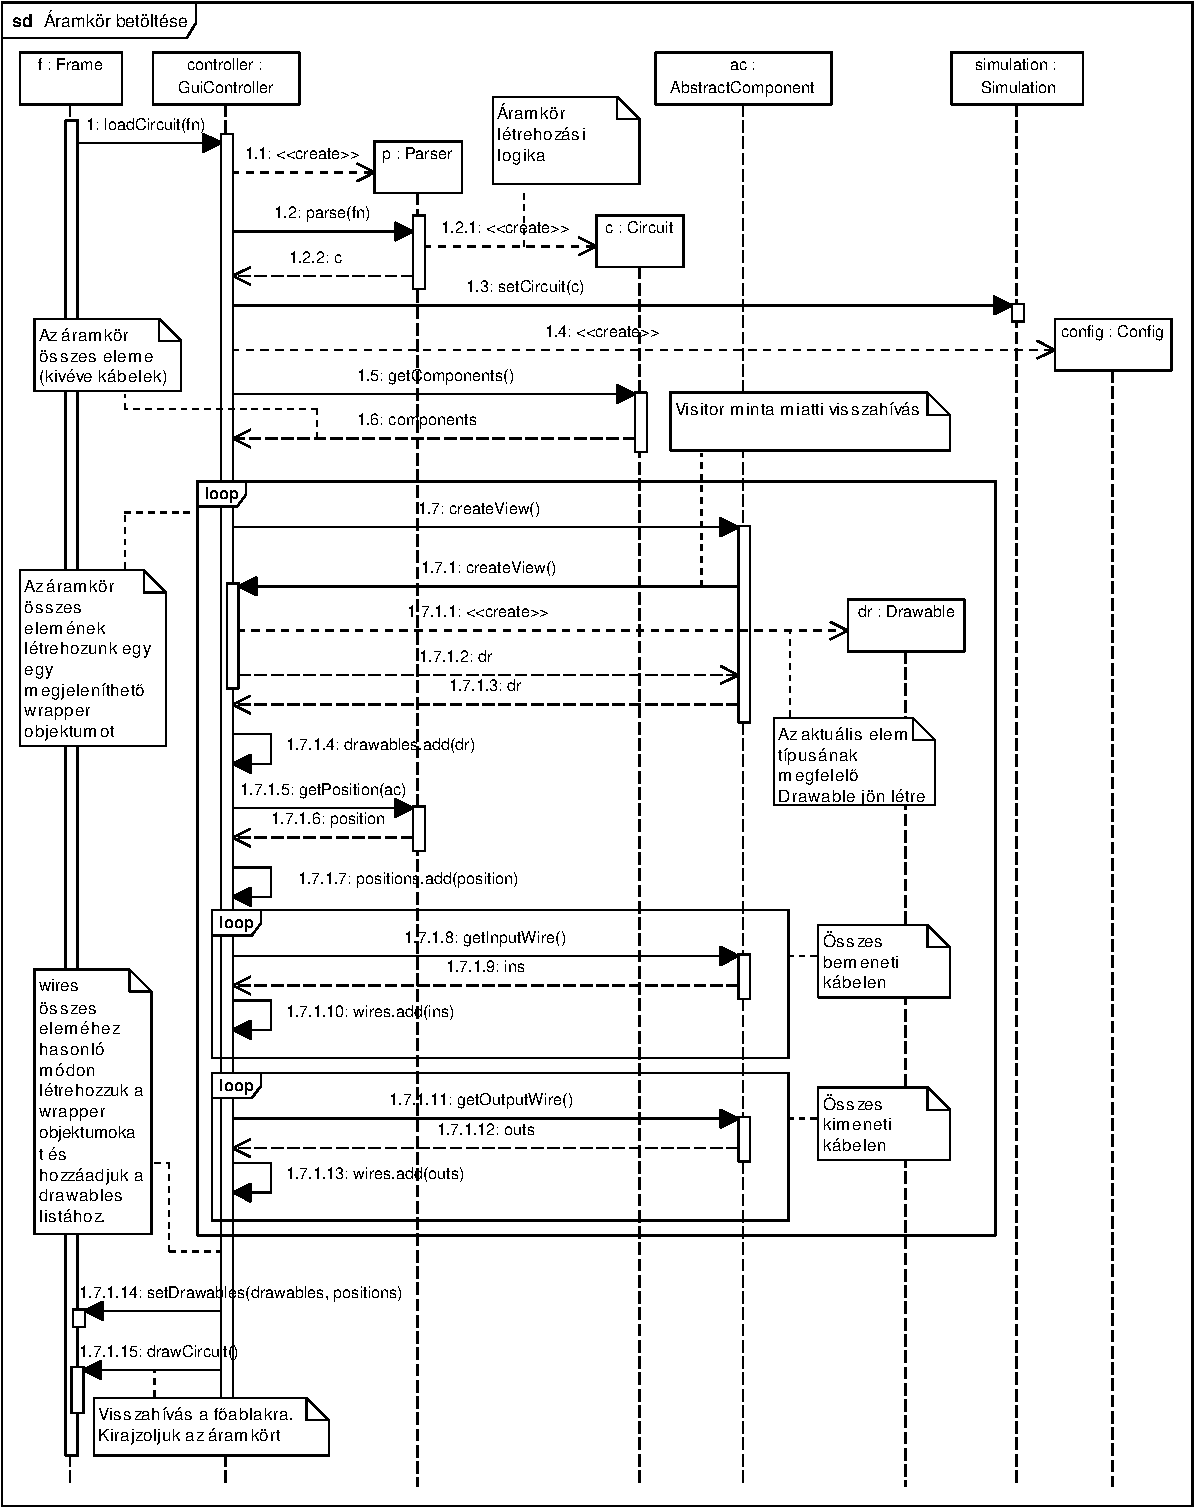
\includegraphics[width=17cm]{chapters/chapter11/pdfs/2_loadcircuit.pdf}
\caption{Áramkör betöltése}
\label{fig:loadcircuit}
\end{center}
\end{figure}

\begin{figure}[h]
\begin{center}
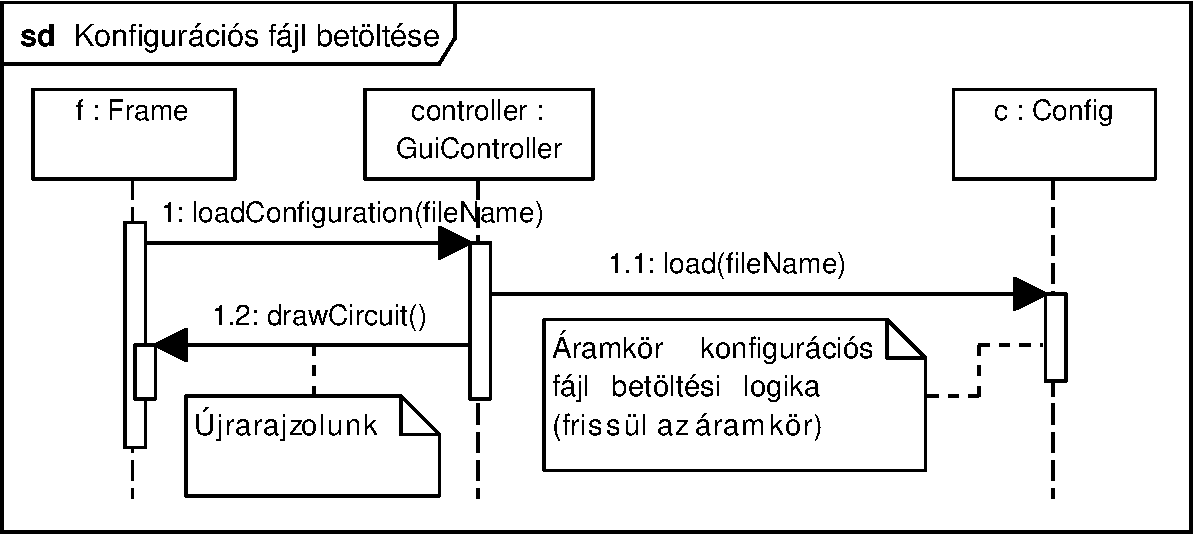
\includegraphics[width=17cm]{chapters/chapter11/pdfs/3_loadconfig.pdf}
\caption{Konfigurációs fájl betöltése}
\label{fig:loadconfig}
\end{center}
\end{figure}

\begin{figure}[h]
\begin{center}
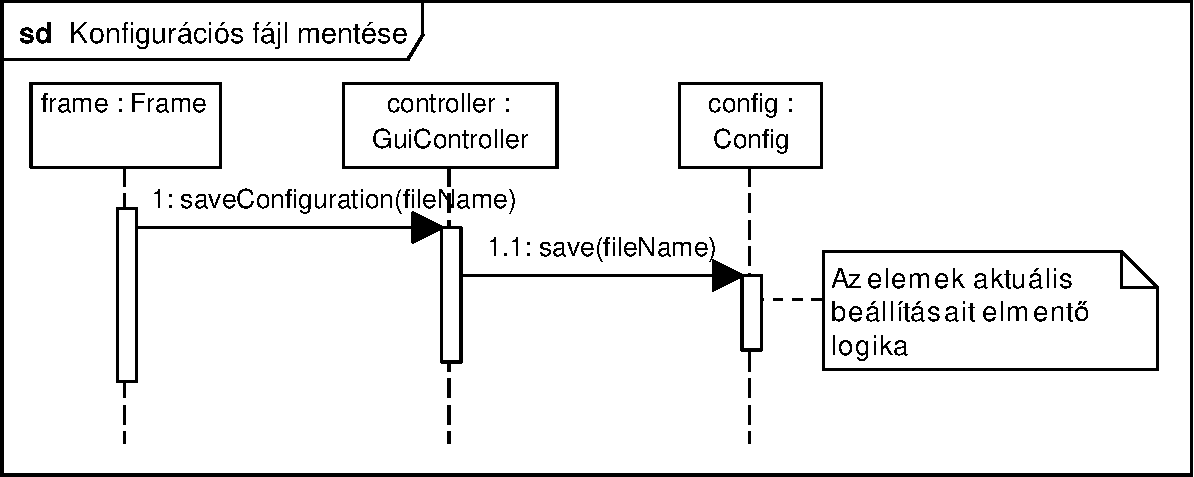
\includegraphics[width=17cm]{chapters/chapter11/pdfs/4_saveconfig.pdf}
\caption{Konfigurációs fájl mentése}
\label{fig:saveconfig}
\end{center}
\end{figure}

\begin{figure}[h]
\begin{center}
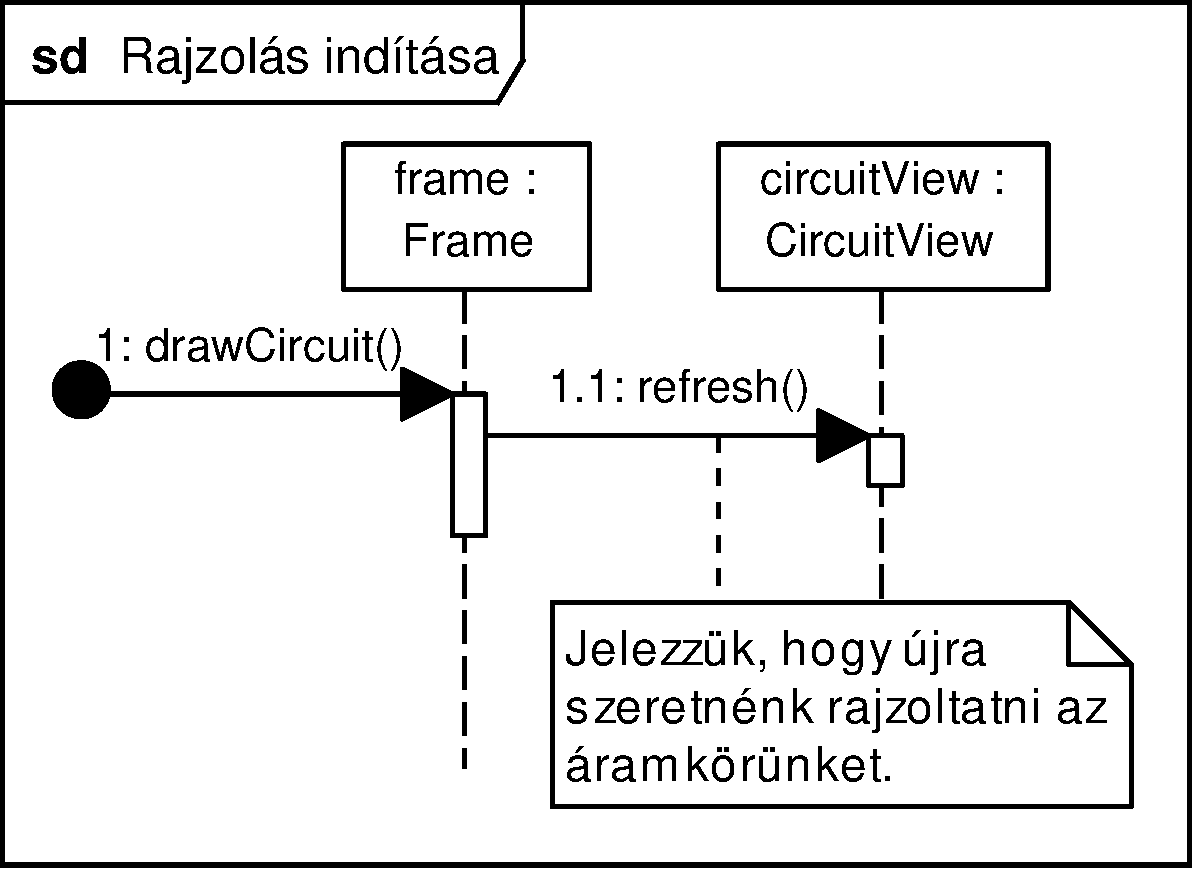
\includegraphics[width=10cm]{chapters/chapter11/pdfs/5_paint1.pdf}
\caption{Rajzolás indítása}
\label{fig:paint1}
\end{center}
\end{figure}

\begin{figure}[h]
\begin{center}
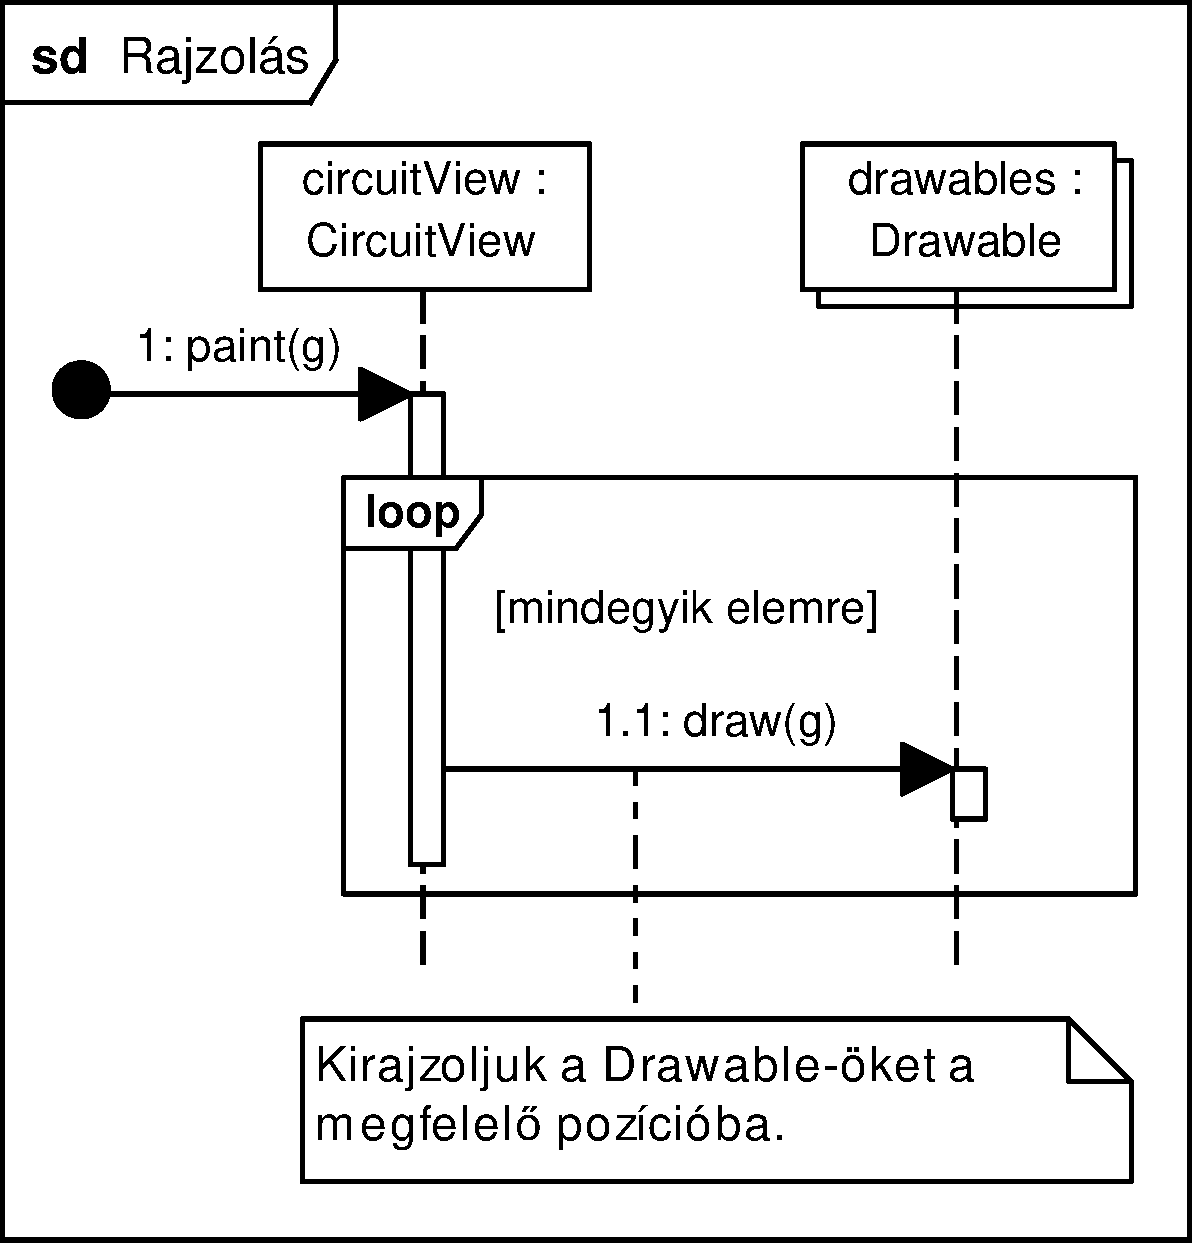
\includegraphics[width=10cm]{chapters/chapter11/pdfs/6_paint2.pdf}
\caption{Rajzolás}
\label{fig:paint2}
\end{center}
\end{figure}

\begin{figure}[h]
\begin{center}
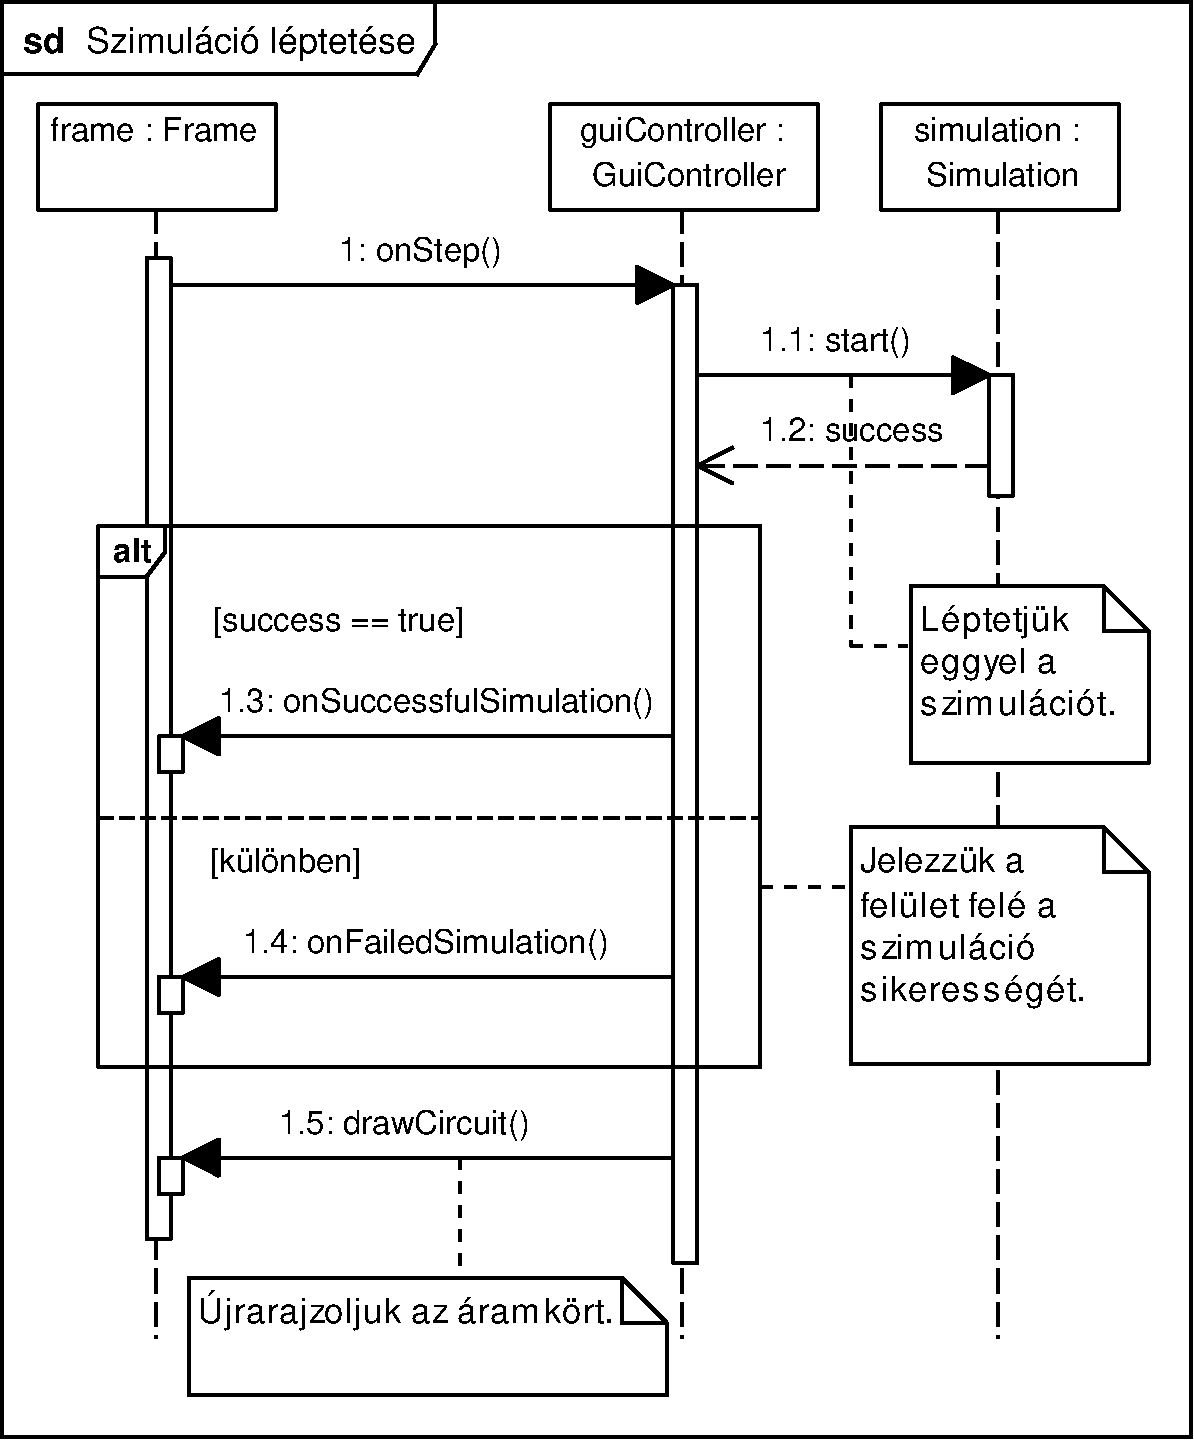
\includegraphics[width=15cm]{chapters/chapter11/pdfs/7_step.pdf}
\caption{Szimuláció léptetése}
\label{fig:step}
\end{center}
\end{figure}

\begin{figure}[h]
\begin{center}
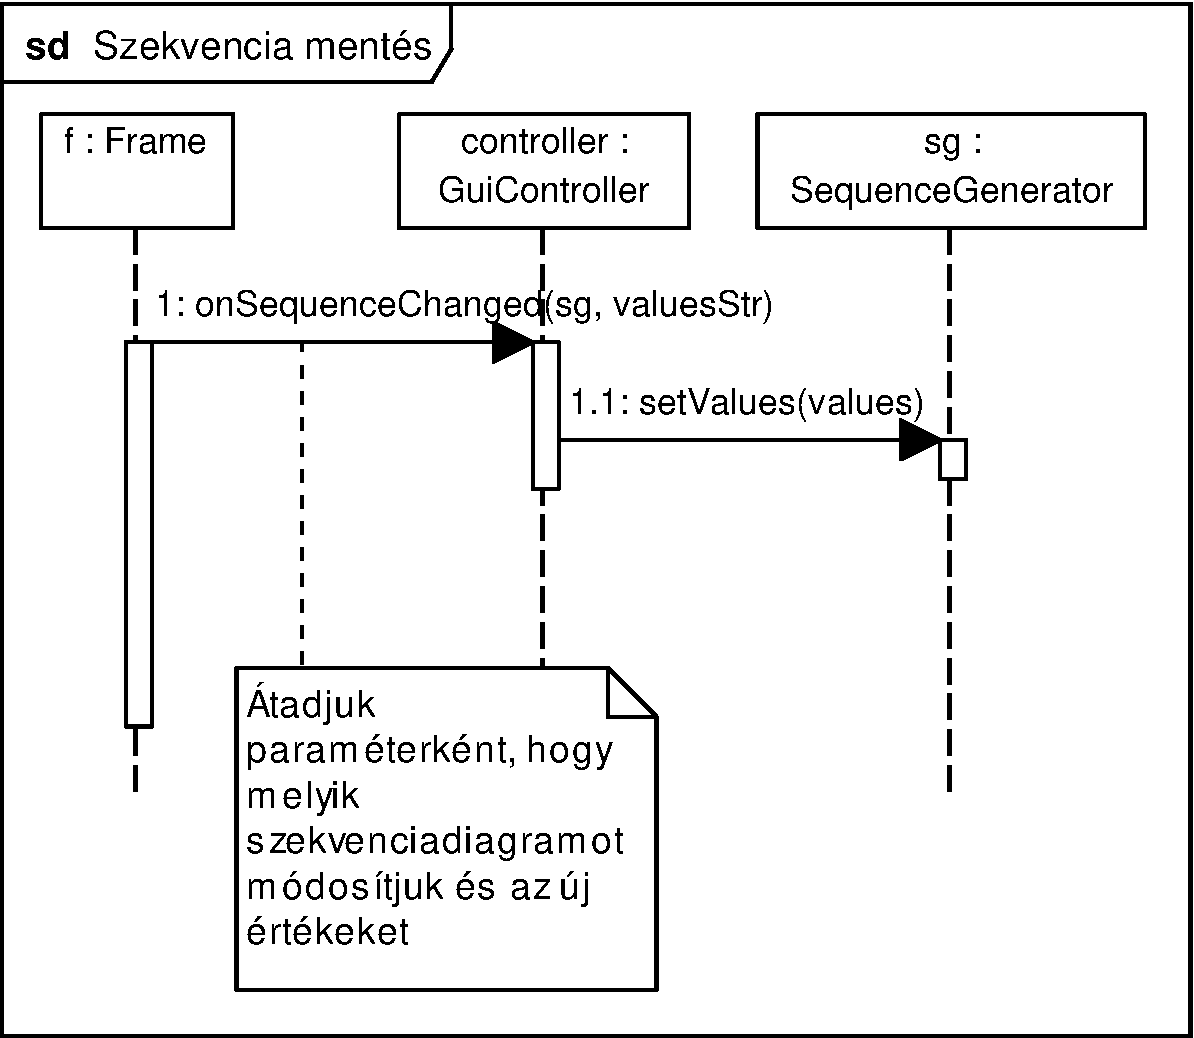
\includegraphics[width=10cm]{chapters/chapter11/pdfs/8_newsequence.pdf}
\caption{Szekvencia mentése}
\label{fig:newsequence}
\end{center}
\end{figure}

\begin{figure}[h]
\begin{center}
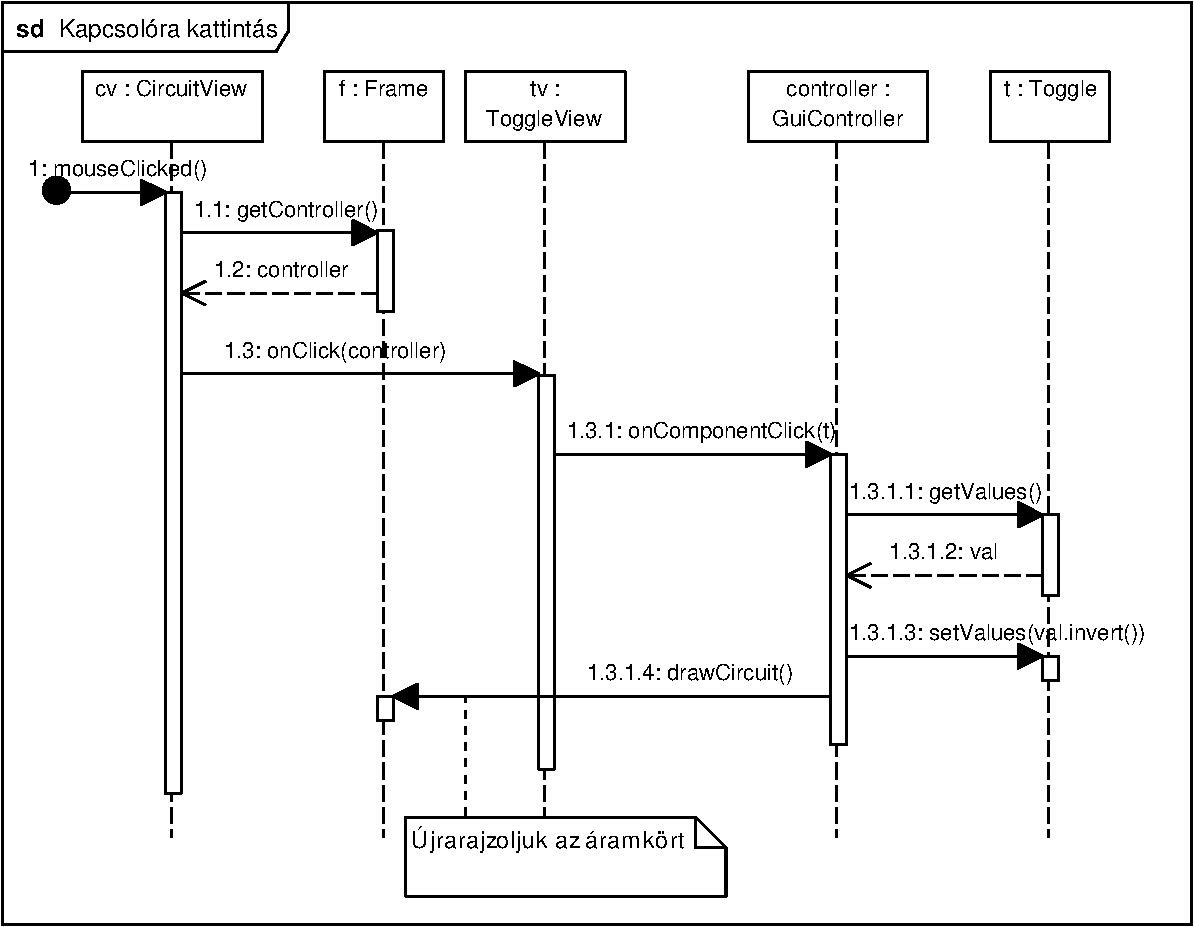
\includegraphics[width=17cm]{chapters/chapter11/pdfs/9_toggle.pdf}
\caption{Kapcsolóra kattintás}
\label{fig:toggle}
\end{center}
\end{figure}

\begin{figure}[h]
\begin{center}
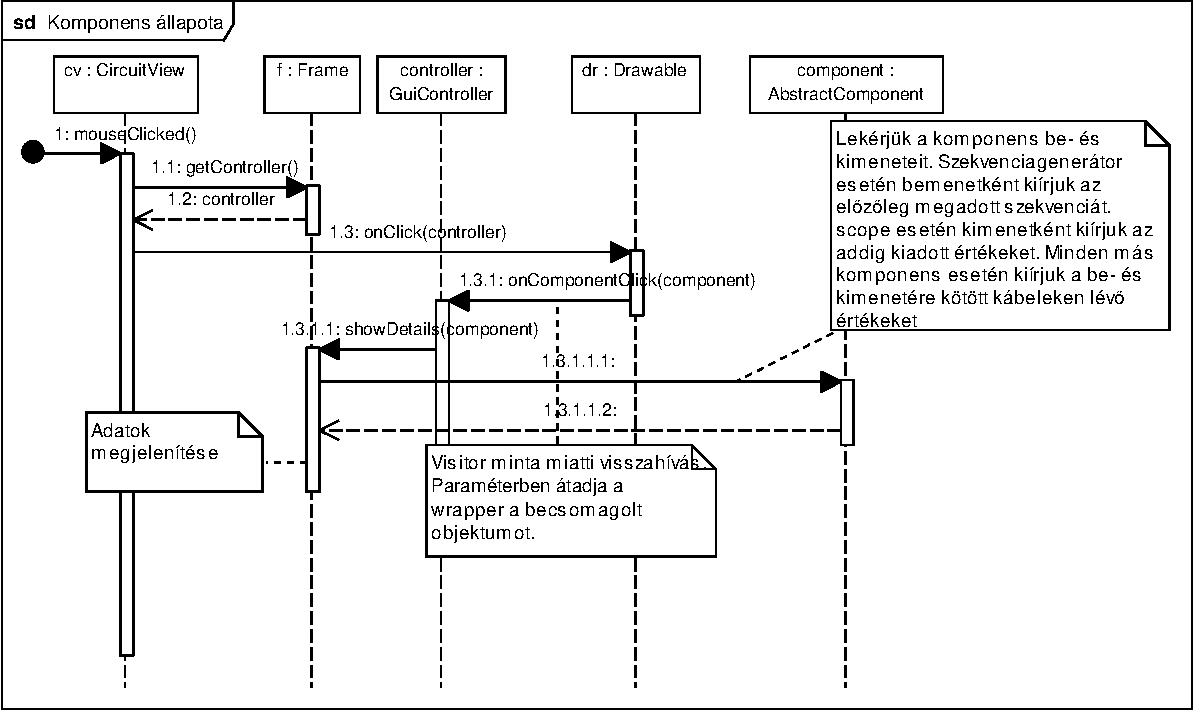
\includegraphics[width=17cm]{chapters/chapter11/pdfs/10_showcomponent.pdf}
\caption{Komponens állapotának kijelzése}
\label{fig:showcomponent}
\end{center}
\end{figure}

\begin{figure}[h]
\begin{center}
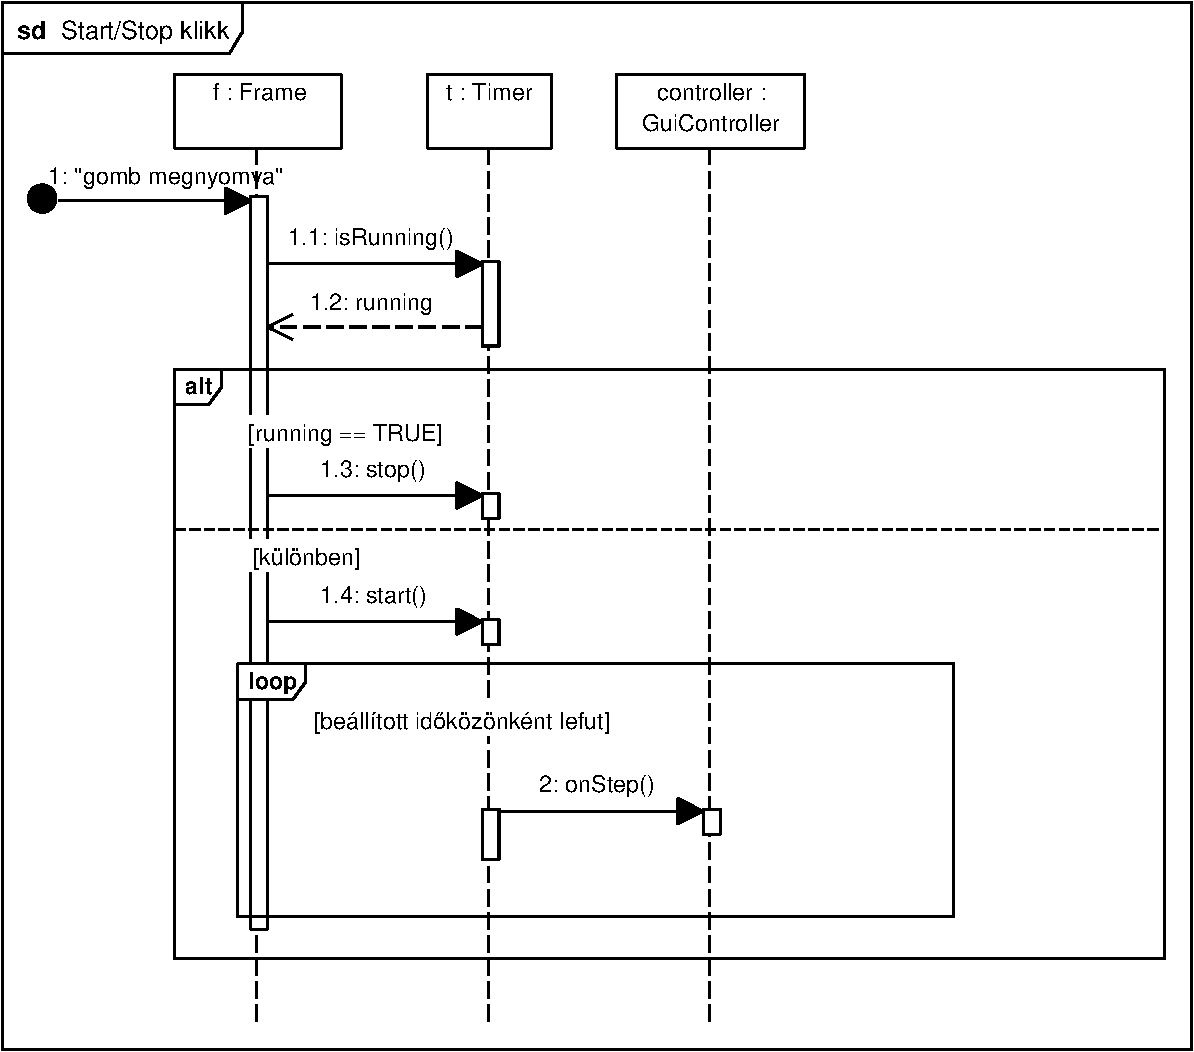
\includegraphics[width=17cm]{chapters/chapter11/pdfs/11_startstop.pdf}
\caption{Start/Stop klikk}
\label{fig:startstop}
\end{center}
\end{figure}

\begin{figure}[h]
\begin{center}
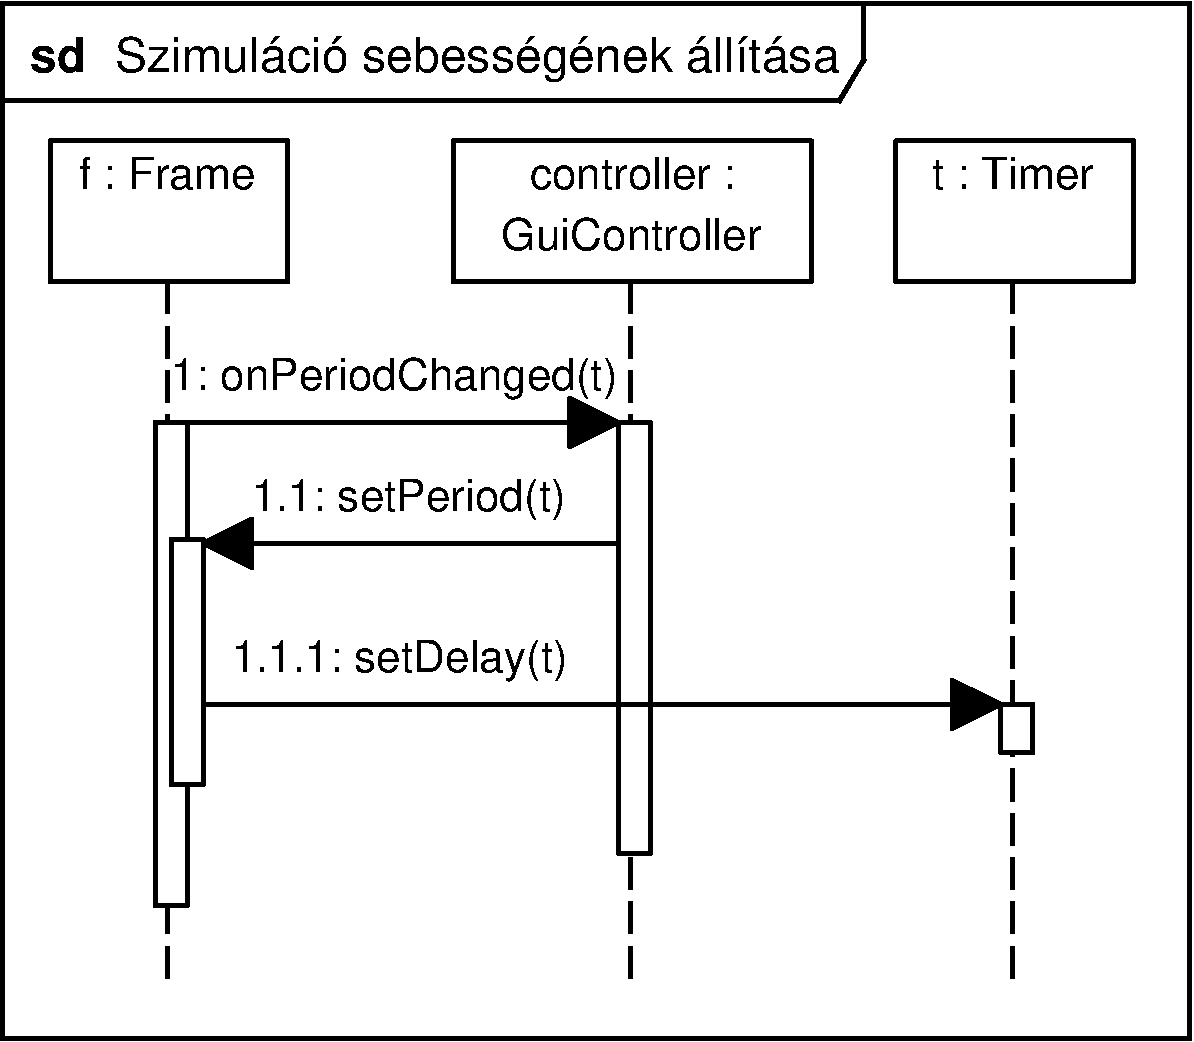
\includegraphics[width=6cm]{chapters/chapter11/pdfs/12_szimseb.pdf}
\caption{Szimuláció sebességének állítása}
\label{fig:szimseb}
\end{center}
\end{figure}